\chapter{実験}
ここでは本研究において行った実験について述べる.

\section{実験1ドライブレコーダー映像を利用した実験}
\subsection{実験内容}
本研究における最初の本実験として、予備実験をもとに実装したシステムを実際にドライブレコーダー映像を使って検証した。
また、strct2depth画面における車のbbox内のG値が100を超えた際に渋滞と判断し、画面左上に「Traffic Jam」という文字列が表示されるようにした。
加えて、映像中に渋滞が判断された回数をフレームごとにJam Counterとして回数を映像中段左に表示されるようにした。

\subsection{使用したデータセット}
本実験にて使用したデータセットは動画投稿サイトYouTubeにて公開されていた高速道路を走行中の映像に加え、私の家族が使用している自家用車に取り付けられたドライブレコーダー映像を用いる。
どの映像も30秒から1分のものであり、常に先行車がある映像を使用した。以下に使用した映像について表で示す。

% ----------------------------------------------------
\begin{table}[htbp]
  \centering
  \begin{scriptsize}
  \begin{tabular}{ccccc}
  \toprule
映像番号 & 時間帯 & 撮影場所 & 車線数 & 動画時間\\
  \midrule
映像1 & 昼間 & 一般道 & 1 & 1分\\
映像2 & 昼間 & 一般道 & 2 & 1分\\
映像3 & 不明 & 高速道路(トンネル) & 2 & 1分 \\
映像4 & 夜間 & 高速道路 & 3 & 30秒\\
  \bottomrule
  \end{tabular}
  \end{scriptsize}
  \caption{使用したデータセット}
  \label{tab:dataset}
\end{table}
% ------------------------------------------------------
\newpage
% 実験1で発生した問題を述べる
\section{実験結果と課題}
ここでは実験1における実験結果について問題と考察を述べる.
まず、実験1における実験結果の一部を以下に示す。
実験結果1〜3の通り、予備実験にて改良したシステムをそのまま用いると、様々な状況で渋滞を誤検出するという問題が発生してしまう。

% --------------------------------------------------
\begin{figure}[htbp]
  \begin{tabular}{c}
    \begin{minipage}{0.33\hsize}
      \begin{center}
   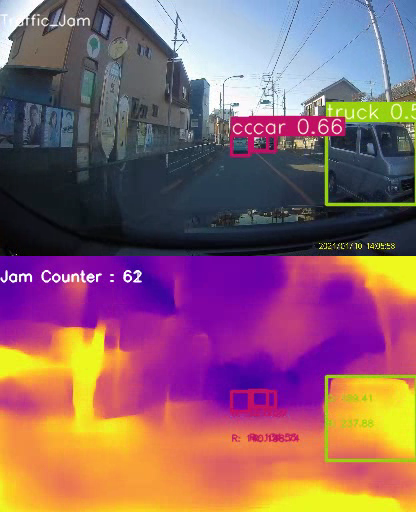
\includegraphics[width=4.5cm]{figs/ex01_01.png}
    \end{center}
  \caption{結果1}
  \label{fig:ex01_01}
\end{minipage}

  \begin{minipage}{0.33\hsize}
  \begin{center}
    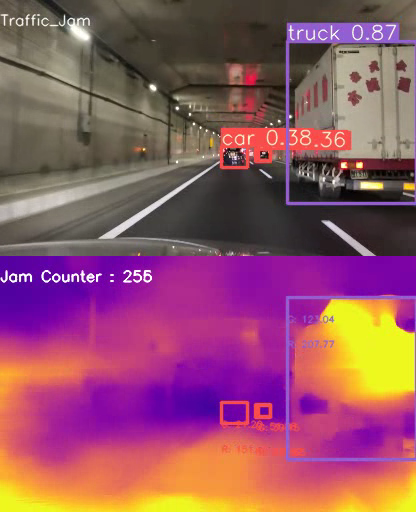
\includegraphics[width=4.5cm]{figs/ex01_02.png}
  \end{center}
  \caption{結果2}
  \label{fig:ex01_02}
\end{minipage}

  \begin{minipage}{0.33\hsize}
  \begin{center}
    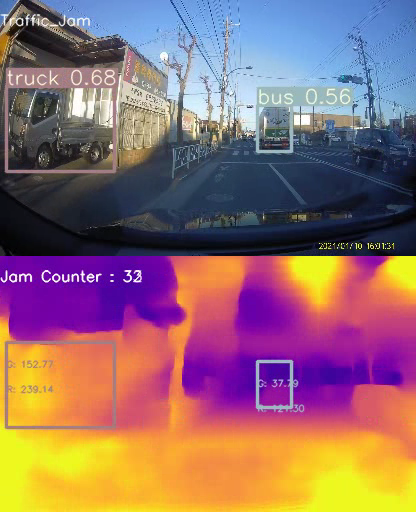
\includegraphics[width=4.5cm]{figs/ex01_03.png}
  \end{center}
  \caption{結果3}
  \label{fig:ex01_03}
\end{minipage}
\end{tabular}
\end{figure}
% ---------------------------------------------------
\figref{fig:ex01_01},\figref{fig:ex01_02},および\figref{fig:ex01_03}の結果からわかるように様々な要因で渋滞の誤検出が起きた。
まず、\figref{fig:ex01_01}においては対向車がドライブレコーダー付きの自動車を横切ってしまうとその際に渋滞と判断してしまう例である。
対向車の存在は渋滞と関係ないのに対し、渋滞と判断してしまうのは正しい判断ではない。
次に、\figref{fig:ex01_02}においては、複数車線がある場合に隣の車線の自動車が近くで走行している際に渋滞だと判断してしいる例である。
先述の対向車のケースとは異なり、隣の車線の混雑は走行車線の混雑と関係がある。
しかし、\figref{fig:ex01_02}のように、先行車との距離があるにもかかわらずたまたま隣で走っていたトラックが近いがために渋滞だと判断してしまうのは正しい判断ではない。
そして、\figref{fig:ex01_03}においては、道路脇に駐車しているトラックを画像検知システムが検知してしまい、渋滞だと判断している例である。
高速道路では稀であるが一般道を走行している際に道路脇に自動車が駐車されているのは珍しいことではなく、またその駐車は渋滞には一切関係がない。
それにもかかわらず渋滞だと判断しているのは正しい判断ではない。
これらの判断ミスのケースは\tabref{tab:dataset}の表にある映像のいずれにおいても頻繁に発生する問題であった。

\subsection{解決アプローチ}
問題の解決のために対向車、隣車線の自動車および駐車している自動車を検出しないという解決策を取った。


\section{実験2}

\section{実験結果}


